\section{Estudio de la estabilidad}

El control de la estabilidad en los robots bípedos resulta muy complejo. Para solucionarlo muchos investigadores han simplificado el cuerpo del robot. 

En este capítulo se van a explicar las dos simplificaciones más utilizadas a la hora de estudiar la estabilidad de los robots humanoides bípedos, y más en concreto la estabilidad del robot TEO utilizado en el actual proyecto.



\subsection{Modelo Péndulo Invertido Lineal}

La primera de ellas es el modelo del péndulo invertido lineal (LIPM)%%abreviatura.
. Éste es el modelo más básico utilizado para simplificar la cinemática y la dinámica de los robots bípedos. Se trata de un modelo desarrollado en dos dimensiones con uno (una única unión rotacional)o dos (incluyendo una unión lineal) grados de libertad. S. Kajita (%añadir la citación de introduction to humanoid robotics
) llegó a este modelo haciendo tres suposiciones. La primera de ellas es que la masa total del robot está concentrada en el CoM. En la segunda supone que el robot tiene piernas sin masa, cuyas puntas entran en contacto con el suelo a través de puntos de rotación individuales. Y la última considera que el robot se mueve solamente en el plano sagital (mostrado en la figura \ref{figura41}).

\begin{figure}[H]
\centering
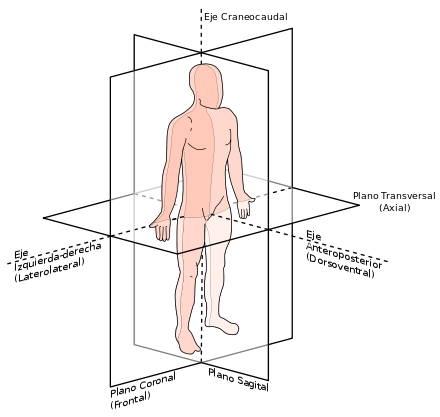
\includegraphics[scale=0.6]{imagenes/apartado_4/41_plano_anatomico_sagital3}
\caption{Planos Anatómicos}
\label{figura41}
\end{figure}

\begin{figure}[H]
\centering
\subfigure[1 grado de libertad]
{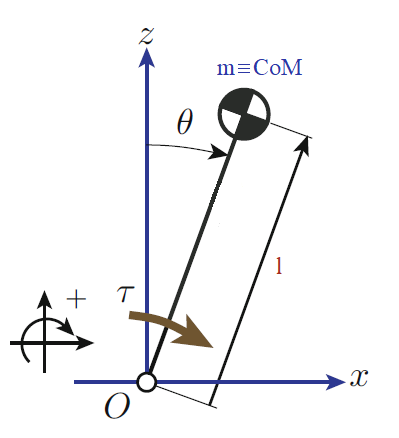
\includegraphics[scale=0.65]{imagenes/apartado_4/42_1_Linear_Inverted_Pendulum_Model_LIPM}}
\quad
\subfigure[2 grados de libertad]
{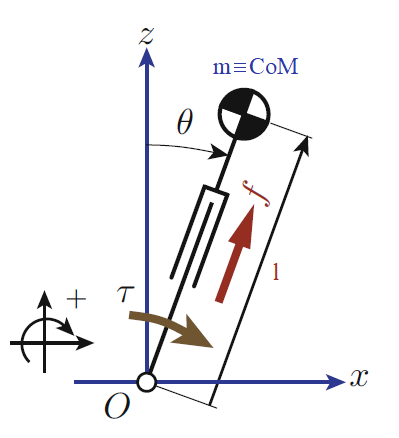
\includegraphics[scale=0.65]{imagenes/apartado_4/42_2_Linear_Inverted_Pendulum_Model_LIPM}}
\caption{Modelo Péndulo Invertido Lineal}
\label{figura42}
\end{figure} 

La ecuación que define el movimiento del CoM es la siguiente:

\begin{equation}
\tau = - ml^2\ddot{\theta}+mgl\sin\theta
\label{ec41}
\end{equation}

donde $m$ es la masa del sistema localizada en el CoM, $l$ es la longitud del péndulo, $\tau$ es el par en el punto de rotación y $\theta$ es el ángulo del péndulo. Sin embargo, esta es una ecuación no lineal, por lo que resulta en un controlador muy complejo para el robot. Para resolver este problema asumimos que $\theta$ es lo suficientemente pequeño ($\theta<10º$) como para considerar que $\sin\theta=\theta$. Esta simplificación le permitió a Kajita (%%%kajita model 3d 2001)
) desarrollar el modelo más utilizado a lo largo de los años para el estudio de la estabilidad de los robots bípedos, una evolución del modelo lineal en 2D, que le permitió trabajar en 3D, el modelo Péndulo Invertido Lineal en tres dimensiones (3DLIPM%%%%acrónimos)
)\cite{ref15}.

\begin{figure}[H]
\centering
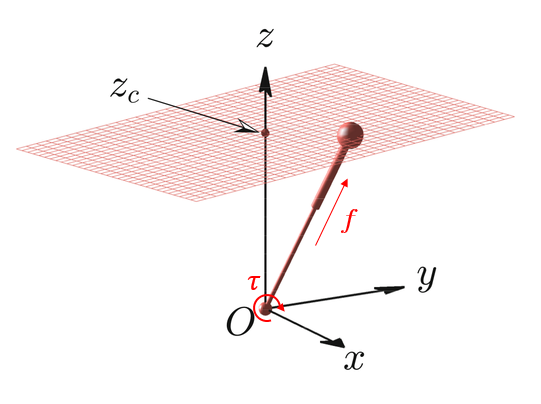
\includegraphics[scale=0.5]{imagenes/apartado_4/43_3D_linear_inverted_pendulum_model}
\caption{Modelo Péndulo Invertido Lineal 3D (3DLIPM)}
\label{figura43}
\end{figure}

Tras la simplificación la ecuación \ref{ec41} queda:

\begin{equation}
\tau = - ml^2\ddot{\theta}+mgl\theta
\label{ec42}
\end{equation}

La posición del CoM $\textbf{p}=(x,y,z)$ está determinada por unas variables de estado $\textbf{q}=(\theta_r,\theta_p,r)$, luego las ecuaciones en los 3 ejes quedan:

\begin{equation}
x=rS_p
\label{ec43}
\end{equation}
\begin{equation}
y=-rS_r
\label{ec44}
\end{equation}
\begin{equation}
z=rD
\label{ec45}
\end{equation}

donde $S_r \equiv \sin\theta_r; S_p \equiv \sin\theta_p; D \equiv \sqrt{1-S_r^{2}-S_p^{2}}$.

Teniendo en cuenta que $(\tau_r,\tau_p,f)$ son los pares y fuerzas asociados a las variables de estado $(\theta_r,\theta_p,r)$, la ecuación del movimiento del péndulo invertido 3D queda descrita matemáticamente como:

\begin{equation}
m\begin{pmatrix}
\ddot{x}\\ 
\ddot{y}\\ 
\ddot{z}
\end{pmatrix}=\left (J^{T} \right )^{-1}\begin{pmatrix}
\tau_r\\ 
\tau_p\\ 
f
\end{pmatrix}+\begin{pmatrix}
0\\ 
0\\ 
-mg
\end{pmatrix}
\label{ec46}
\end{equation}

donde la estructura de la jacobiana es:

\begin{equation}
J=\frac{\partial p}{\partial q}=\begin{pmatrix}
0 & rC_p & S_p\\ 
-rC_r & 0 & -S_r\\ 
-rC_rS_r/D &-rC_pS_p/D  & D
\end{pmatrix}
\label{ec47}
\end{equation}

\begin{equation}
C_r \equiv \cos\theta_r, C_p \equiv \cos\theta_p
\label{ec48}
\end{equation}

\begin{equation}
S_r \equiv \sin\theta_r, S_p \equiv \sin\theta_p
\label{ec49}
\end{equation}

\begin{equation}
D \equiv \sqrt{1-S_r^{2}-S_p^{2}}
\label{ec410}
\end{equation}

Sustituyendo \ref{ec43}, \ref{ec44} y \ref{ec45}, se obtienen las ecuaciones de la dinámica en los ejes $x$, $y$ y $z$

\begin{equation}
m\left ( -z\ddot{y} - y\ddot{z} \right ) = \frac{D}{C_r}\tau_r - mgy
\label{ec411} 
\end{equation}

\begin{equation}
m\left ( -z\ddot{x} - x\ddot{z} \right ) = \frac{D}{C_p}\tau_p - mgx
\label{ec412} 
\end{equation}

\begin{equation}
m\left ( -x\ddot{x} + y\ddot{y} + z\ddot{z} \right ) = rf - mgz
\label{ec413} 
\end{equation}

Pero estas ecuaciones del péndulo invertido son no lineales y demasiado complejas para usarlas en la generación de tareas de caminata. Por esta razón se restringe el movimiento del CoM en la coordenada z al plano $Z_c$, cuyo vector normal es $(k_x,k_y,-1)$.

\begin{equation}
z = k_x x + k_y y + z_c
\label{ec414}
\end{equation}

%%esto está sacado de: https://www.techunited.nl/media/files/humanoid/SwanVanDalen_GRAD2012_A_Linear_Inverted_Pendulum_Walk_Implemented_on_TUlip.pdf

Si el plano de restricción es horizontal $(k_x=k_y=0)$, la dinámica bajo el control de la restricción están dada por

\begin{equation}
\ddot{x}=\frac{g}{z_c}x - \frac{1}{m z_c}\tau_y
\label{ec415}
\end{equation}

\begin{equation}
\ddot{y}=\frac{g}{z_c}y - \frac{1}{m z_c}\tau_x
\label{ec416}
\end{equation}

\begin{equation}
\ddot{z}=0
\label{ec417}
\end{equation}

En el caso de que el plano de restricción esté inclinado ($k_x=k_y\neq0$), se puede obtener la misma dinámica aplicando una restricción adicional para los pares de entrada,

\begin{equation}
\tau_{x} x + \tau_{y} y = 0
\label{ec418}
\end{equation}

A partir del modelo 3DLIPM junto a la restricción horizontal $(k_x=k_y=0)$ podemos obtener la posición de la proyección del Punto de Momento Cero (ZMP) en el suelo,

\begin{equation}
x_{ZMP} = -\frac{\tau_y}{mg}
\label{ec419}
\end{equation}

\begin{equation}
y_{ZMP} = -\frac{\tau_x}{mg}
\label{ec420}
\end{equation}



%%eSTO LO HE SACADO DE kajita2003preview_models_inverted_pendulum_cart_table

\subsubsection{LIPM aplicado al robot humanoide TEO}

Los sensores que se han utilizado son los F-T de los tobillos, ya que son los que están en contacto con el suelo. Gracias a su información se puede calcular la posición del ZMP para que TEO pueda conservar el equilibrio, a partir de las ecuaciones del modelo de péndulo invertido 3DLIPM. 

Las ecs. \ref{ec419} y \ref{ec420} del ZMP para este modelo responden a la ecuación general:

\begin{equation}
x_{ZMP}=-\frac{\sum x\cdot F_z}{\sum F_z}
\label{ec421}
\end{equation}

Pero este modelo se ha tenido que modificar para el robot TEO utilizado en el actual proyecto, ya que se considera que cuando un robot bípedo está soportando su peso en un pie, el tobillo del robot se convierte en el punto pivotante del modelo conectado al CoM del robot a través de su pierna sin masa. Pero este punto pivotante no se encuentra totalmente en el suelo ya que la estructura de TEO está construida de tal manera que el tobillo está elevado respecto al suelo debido a la anchura de la suela del robot, como se muestra en la figura \ref{figura51}. Por lo tanto, la ec. del ZMP adaptada sería:

\begin{equation}
x_{ZMP}=-\frac{\tau_y + h F_x}{F_z}
\label{ec422}
\end{equation}

donde $\tau_y$ es el par en el punto pivotante alrededor del eje $y$, $F_x$ y $F_z$ son las fuerzas medidas en las direcciones $x$ y $z$ respectivamente, y $h$ es la altura de la suela del robot hasta la localización del sensor F-T.

\begin{figure}[H]
\centering
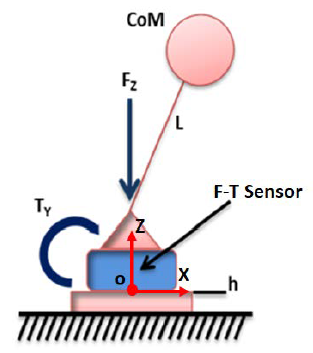
\includegraphics[scale=0.8]{imagenes/apartado_4/44_LIPM_TEO}
\caption{Modelo LIPM con un sensor F-T entre el tobillo y la suela}
\label{figura44}
\end{figure}

Pero esta ecuación sólo valdría cuando el robot está apoyado sobre una pierna (simple apoyo). Sin embargo, el proyecto se ha desarrollado estando apoyadas las dos piernas (doble apoyo), por lo que la ecuación para el ZMP global es:


\begin{equation}
x_{ZMP_{DS}}=\frac{x_{ZMP}^{R}F_{z}^{R}+x_{ZMP}^{L}F_{z}^{L}}{F_{z}^{R}+F_{z}^{L}}
\label{ec423}
\end{equation}

donde R indica la pierna derecha y L la pierna izquierda. A pesar de que en doble apoyo el robot tiene dos puntos pivotantes en los tobillos, se puede aplicar el modelo de péndulo invertido simple ya que ambos tobillos tienen el mismo movimiento a lo largo del eje $x$ (plano sagital).

\subsubsection{DLIPM: mejora del modelo del péndulo invertido simple}\label{definicionDLIPM}

En la respuesta dinámica del modelo de péndulo invertido simple se observaba que había cierto error conforme se aumentaba el ZMP. Ésto se corrigió en \cite{ref21} con una mejora de dicho modelo en la respuesta dinámica eliminando ese error, es decir, ajustando el ZMP calculado a partir de los datos obtenidos de los sensores F-T de los tobillos a un ZMP teórico al que debería llegar el robot. Este modelo se denomina DLIPM.

\begin{figure}[H]
\centering
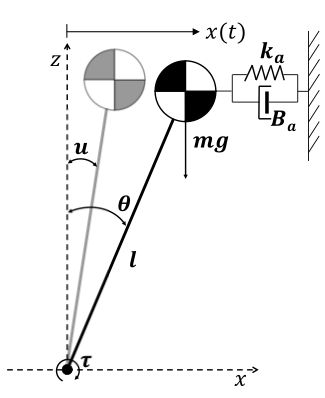
\includegraphics[scale=0.45]{imagenes/apartado_4/45_modelo_dlipm}
\caption{Modelo DLIPM}
\label{figura45}
\end{figure}

Esta mejora consiste en la adición de un muelle $k_a$ y un amortiguador $B_a$ (figura \ref{figura45}) para compensar la respuesta del estado estacionario ($k_a$) y la respuesta del régimen transitorio para limitar las oscilaciones ($B_a$) del sistema LIPM.

La ecuación del movimiento de dicho modelo estaría dada por:

\begin{equation}
\tau = -ml\ddot{x}(t) - B_a l\dot{x}(t) - k_a lx(t) + mgx(t)
\label{ec424}
\end{equation}

donde $x(t)$ indica el movimiento del CoM, $m$ es la masa del péndulo localizada en el CoM, $l$ la longitud del péndulo, $k_a$ la constante del muelle y $B_a$ la constante del amortiguador. El desplazamiento del CoM es tan pequeño que se puede asumir que $\sin\theta = \theta$, quedando la ecuación 4.24 como:

\begin{equation}
\tau = -ml\ddot{\theta}(t) - B_a l\dot{\theta}(t) - k_a l\theta(t) + mg\theta(t)
\label{ec425}
\end{equation}

Por otra parte, el par también se puede obtener de la medición del ZMP como:

\begin{equation}
\tau = - x_{FT} \cdot mg
\label{ec426}
\end{equation}

donde $x_{FT}$ es la coordenada x del ZMP medido por los sensores de los tobillos. Combinando \ref{ec425} y \ref{ec426} se obtiene:

\begin{equation}
- x_{FT} \cdot mg = -ml\ddot{\theta}(t) - B_a l\dot{\theta}(t) - k_a l\theta(t) + mg\theta(t)
\label{ec427}
\end{equation}

Siendo ésta la ecuación que explica la física del modelo DLIPM que se ha desarrollado en el actual proyecto.

\newpage

\subsection{Modelo cart-table}

La siguiente simplificación más utilizada para el control del equilibrio de los robots humanoides bípedos es el modelo cart-table.

Este modelo proporciona información de las aceleraciones e inercias del cuerpo del robot, muy útiles a la hora de realizar tareas de caminata dinámica. Consiste en un carro de masa M corriendo sobre una mesa sin masa (figura \ref{figura46}). Tiene la misma dinámica de movimiento que el modelo de péndulo invertido pero añade una relación directa entre el ZMP y el movimiento.

\begin{figure}[H]
\centering
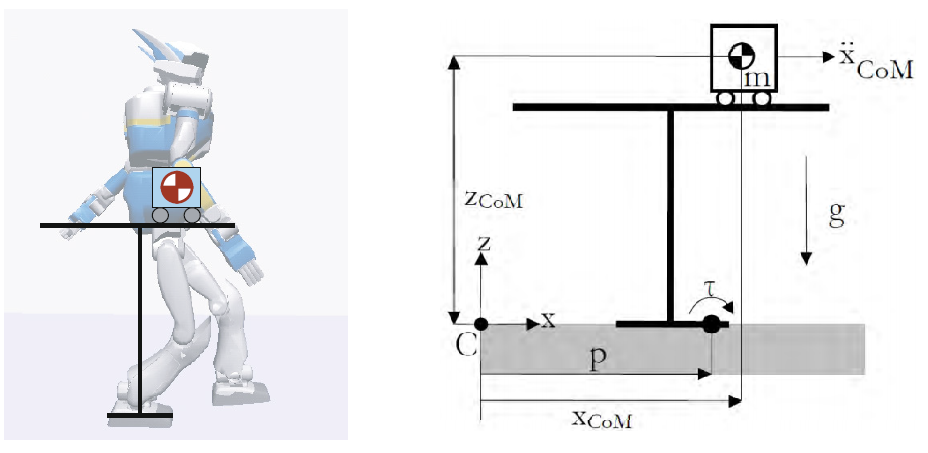
\includegraphics[scale=0.5]{imagenes/apartado_4/46_cart_table_model_2}
\caption{Modelo Cart-Table}
\label{figura46}
\end{figure}

Las ecuaciones del modelo cart-table para controlar el ZMP se obtienen sustituyendo \ref{ec419} y \ref{ec420} en \ref{ec415} y \ref{ec416} del modelo 3DLIPM,

\begin{equation}
\ddot{x}_{CoM}=\frac{g}{z_{CoM}}\left ( x_{CoM} - x_{ZMP} \right )\Rightarrow x_{ZMP} = x-\frac{z_{CoM}}{g}\ddot{x}_{CoM}
\label{ec430}
\end{equation}

\begin{equation}
\ddot{y}_{CoM}=\frac{g}{z_{CoM}}\left ( y_{CoM} - y_{ZMP} \right )\Rightarrow y_{ZMP} = y-\frac{z_{CoM}}{g}\ddot{y}_{CoM}
\label{ec431}
\end{equation}

Estas ecuaciones se denominan \textbf{Ecuaciones del ZMP}. 

Como se puede observar el pie de la mesa es demasiado pequeño para que el carro permanezca en el borde, por lo que el carro debe llevar una determinada aceleración para que la mesa se mantenga en posición vertical durante un tiempo, en el que el ZMP exista dentro del pie de dicha mesa.

Por otro lado Shuuji Kajita y Bernard Espiau \cite{ref20} añadieron que si esta aceleración es demasiado grande, el ZMP calculado se sale del polígono de soporte (\ref{figura46}a). Esto es porque \ref{ec430} y \ref{ec431} no tienen en cuenta el polígono de soporte ni la restricción unilateral (por lo que se asume que el pie está pegado al suelo, y esto no puede ser viable ya que el robot necesita levantar el pie para caminar). Por ello, hay que tener en cuenta dicha restricción, y como se puede observar en la \ref{figura46}b, la mesa ya no está en vertical, por lo que hay que tener en cuenta la aceleración en z a parte de la gravedad, quedando la ecuación del ZMP como:

\begin{equation}
\ddot{x}_{CoM}=\frac{g}{z_{CoM}}\left ( x_{CoM} - x_{ZMP} \right )\Rightarrow x_{ZMP} = x-\frac{z_{CoM}}{g+\ddot{z}_{CoM}}\ddot{x}_{CoM}
\label{ec432}
\end{equation}

que da el cálculo del ZMP en el borde del polígono de soporte (pie de la mesa). 

\begin{figure}[H]
\centering
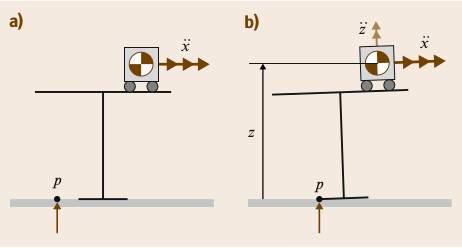
\includegraphics[scale=0.6]{imagenes/apartado_4/47_cart_table_real}
\caption{Cálculo del ZMP. a) Modelo ficticio, b) Modelo real}
\label{figura47}
\end{figure}

Esto es importante ya que un ZMP fuera del polígono de soporte implica que el robot podría no mantener el total contacto pie-suelo y la caminata no se produjese según lo planeado. Cuando el ZMP está dentro del polígono de soporte se puede garantizar el contacto total pie-suelo.

\newpage

\subsection{Equivalencia de modelos}

\begin{comment}

%%Como se puede deducir éstos deben de dar iguales salidas. Pero se observó que ésto no era así, como se puede ver en la figura \ref{figura48}. Por lo que se debían igualar ambos modelos. El procedimiento seguido fue escoger el modelo que más se acercara al ZMP teórico y a partir de ese corregir el otro modelo, por lo que se decidió mejorar el modelo de LIPM y a partir del mismo mejorar la respuesta del cart-table.

\begin{figure}[H]
\centering
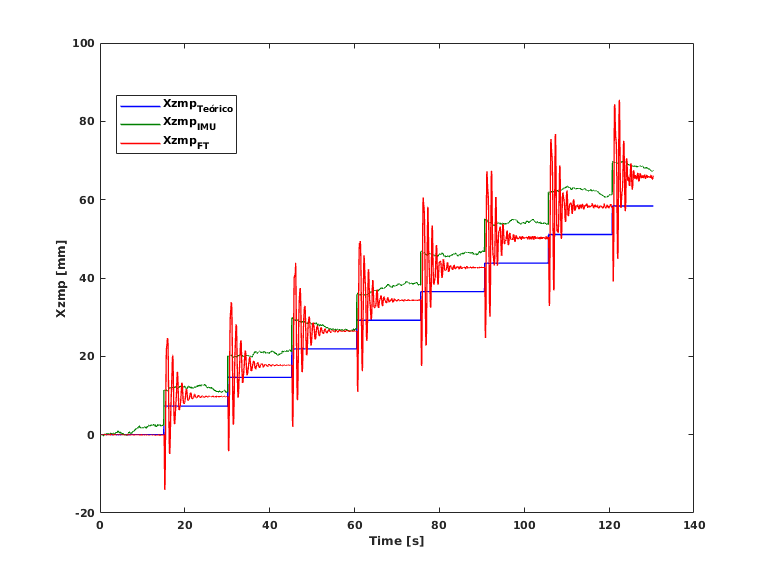
\includegraphics[width=13cm, height=8cm]{imagenes/apartado_4/48_zmp_lipm_cart_table}
\caption{Evolución ZMP modelos LIPM y cart-table}
\label{figura48}
\end{figure}

Para ambos modelos la variable más importante y que tienen en común es la altura del CoM, desde el punto de medida de las fuerzas y los pares para el caso del modelo LIPM (longitud del péndulo), y la longitud desde el suelo hasta el CoM para el modelo cart-table ($Z_{CoM}$). Otra variable que hay que tener en cuenta cuando el robot realiza un paso es la inclinación, ya que ésta varía.

Para el modelo cart-table se necesitan aceleraciones en la dirección en la que se desplaza, por lo que cuando el robot está en posición estática y erguido en doble apoyo no existe dicha aceleración, pero aún así ambos modelos son equivalentes en cualquier instante t, como se puede reflejar en la siguiente ecuación:
\end{comment}

Para ambos modelos la variable más importante y que tienen en común es la altura del CoM, desde el punto de medida de las fuerzas y los pares para el caso del modelo LIPM (longitud del péndulo), y la longitud desde el suelo hasta el CoM para el modelo cart-table ($Z_{CoM}$). Gracias a que la altura del CoM es común en los dos modelos se ha podido desarrollar una equivalencia entre ambos en el actual proyecto.

Esta equivalencia se ha desarrollado tomando como referencia el modelo LIPM (incluyendo sus mejoras), ya que era el modelo que más se acercaba al ZMP deseado en las pruebas realizadas, y a partir del mismo se despejó la altura del CoM del modelo cart-table. 

%%Esta aproximación dió como resultado diferentes alturas para el CoM, esto es debido a que la altura definida para el modelo LIPM no es del todo exacto debido a las diferencias entre los modelos CAD y el modelo real del robot.

Para cualquier instante t durante el paso o en posición estática, los ZMP de ambos modelos coinciden,

\begin{equation}
X_{ZMP_{FT_t}} = X_{ZMP_{IMU_t}} \Leftrightarrow   X_{ZMP_{FT_{(t+1)}}}=X_{ZMP_{IMU_{(t+1)}}}
\label{ec433}
\end{equation}

Por lo tanto:

\begin{equation}
ZMP_{F-T}=ZMP_{IMU}
\label{ec434}
\end{equation}

\begin{equation}
\left.\begin{matrix}
\left.\begin{matrix}
-\frac{\tau+ h F_{x}}{F_{z}}
\end{matrix}\right|_{SS}=X_{CoM}-\frac{Z_{CoM}}{g+\ddot{z}_{CoM}}\ddot{x}_{CoM}
\\ 
\\
\left.\begin{matrix}
\frac{x_{ZMP}^{R}F_{z}^{R}+x_{ZMP}^{L}F_{z}^{L}}{F_{z}^{R}+F_{z}^{L}}
\end{matrix}\right|_{DS}=X_{CoM}-\frac{Z_{CoM}}{g+\ddot{z}_{CoM}}\ddot{x}_{CoM}
\end{matrix}\right\}
\label{ec435}
\end{equation}

donde $x_{CoM}=0$ ya que la referencia del sistema de coordenadas del modelo cart-table siempre es la misma, y por tanto $z_{CoM}$ es constante en todo momento. Como se puede observar el modelo LIPM es equivalente al modelo cart-table tanto en doble como en simple apoyo.

\begin{equation}
x_{ZMP_{F-T}}=-\frac{Z_{CoM}}{g+\ddot{z}_{CoM}}\ddot{x}_{CoM}
\label{ec436}
\end{equation}

Despejando la altura del modelo cart-table e igualando al ZMP del modelo LIPM para que ambos dieran la misma salida de ZMP, ésta quedaría:

\begin{equation}
Z_{CoM}=-\frac{x_{ZMP_{F-T}}(g+\ddot{z}_{CoM})}{\ddot{x}_{CoM}}
\label{ec437}
\end{equation}



\newpage

\subsection{Estrategias de control}

Los seres humanos son capaces de mantener el equilibrio en entornos complejos y novedosos ante diferentes perturbaciones mediante el movimiento de las diferentes partes de su cuerpo. Esta capacidad de respuesta ante perturbaciones externas ha hecho que diferentes investigadores acerquen el estudio de la estabilidad de los seres humanos a los robots humanoides.

Pueden aparecer diferentes perturbaciones que alteren el equilibrio del robot cuando éste se encuentra en una postura estable. Estas perturbaciones pueden aparecer en el plano sagital (perturbaciones anterior-posteriores) o en el plano frontal (perturbaciones mediolaterales). Se han hecho numerosos estudio del equilibrio cuando el robot se encuentra en posición estática, apareciendo diferentes estrategias de control para mantener dicho equilibrio ante la aparición de diferentes perturbaciones. Dichas estrategias se han separado en función de la magnitud de dicha perturbación y de la posición de la postura del robot en: estrategias de tobillo, cadera y paso \cite{ref17} \cite{ref18}.

Estas estrategias están basadas en la cuantificación del cambio de dirección del CoP en las direcciones anteriormente mencionadas.

\begin{figure}[H]
\centering
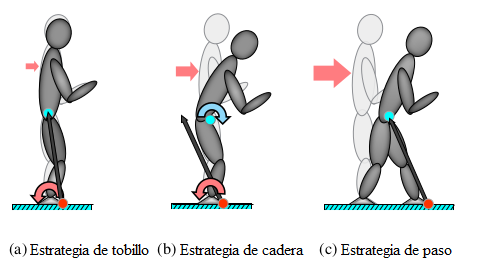
\includegraphics[scale=0.8]{imagenes/apartado_4/49_balance_strategies}
\caption{Estrategias de balance}
\label{figura49}
\end{figure}

La primera de ellas es la estrategia de tobillo. Ésta se aplica para pequeñas perturbaciones anterior-posteriores que tienen lugar en el plano sagital. Se usa para controlar y mantener el CoP en el polígono de soporte. Cuando ocurre una alteración del equilibrio de baja magnitud el cuerpo del robot se puede considerar como un péndulo invertido ajustándose dicho equilibrio mediante el par de la articulación del tobillo. 

En la estrategia de la cadera, al igual que en la estrategia de tobillo, se actúa en el plano sagital y se basa en el balance del CMP. Ésta interviene cuando la perturbación del equilibrio es lo suficientemente intensa como para que la estrategia del tobillo no sea suficiente. Se utiliza la articulación de la cadera y se puede usar independientemente o en combinación con la estrategia del tobillo. 

La última estrategia es la del paso. Ésta se lleva a cabo cuando aparece una perturbación en la que una aplicación de par contraria en las articulaciones no es suficiente para recuperar el equilibrio. Cuando se realiza el paso el área del polígono de soporte se reajusta, creando unos nuevos límites de equilibrio.

Todas ellas dependen de diferentes factores como puede ser las condiciones del entorno (entornos rocosos o lisos, por ejemplo), la forma de la suela del robot, la altura del cuerpo, o la posición en la que se encuentre en el momento en el que se produce dicha perturbación.


\afterpage{\null\newpage}
\newpage